\documentclass[conference]{IEEEtran}

\ifCLASSINFOpdf
   \usepackage[pdftex]{graphicx}
  % declare the path(s) where your graphic files are
   \graphicspath{{./pdf/}{../jpeg/}}
  % and their extensions so you won't have to specify these with
  % every instance of \includegraphics
  \DeclareGraphicsExtensions{.pdf}
\else
  % or other class option (dvipsone, dvipdf, if not using dvips). graphicx
  % will default to the driver specified in the system graphics.cfg if no
  % driver is specified.
  % \usepackage[dvips]{graphicx}
  % declare the path(s) where your graphic files are
  % \graphicspath{{../eps/}}
  % and their extensions so you won't have to specify these with
  % every instance of \includegraphics
  % \DeclareGraphicsExtensions{.eps}
\fi
% graphicx was written by David Carlisle and Sebastian Rahtz. It is
% required if you want graphics, photos, etc. graphicx.sty is already
% installed on most LaTeX systems. The latest version and documentation
% can be obtained at: 
% http://www.ctan.org/pkg/graphicx
% Another good source of documentation is "Using Imported Graphics in
% LaTeX2e" by Keith Reckdahl which can be found at:
% http://www.ctan.org/pkg/epslatex
%
% latex, and pdflatex in dvi mode, support graphics in encapsulated
% postscript (.eps) format. pdflatex in pdf mode supports graphics
% in .pdf, .jpeg, .png and .mps (metapost) formats. Users should ensure
% that all non-photo figures use a vector format (.eps, .pdf, .mps) and
% not a bitmapped formats (.jpeg, .png). The IEEE frowns on bitmapped formats
% which can result in "jaggedy"/blurry rendering of lines and letters as
% well as large increases in file sizes.
%
% You can find documentation about the pdfTeX application at:
% http://www.tug.org/applications/pdftex





\hyphenation{op-tical net-works semi-conduc-tor}


\begin{document}
%
% paper title
% Titles are generally capitalized except for words such as a, an, and, as,
% at, but, by, for, in, nor, of, on, or, the, to and up, which are usually
% not capitalized unless they are the first or last word of the title.
% Linebreaks \\ can be used within to get better formatting as desired.
% Do not put math or special symbols in the title.
\title{Differences in Perceived Merge Conflict Difficulties}

\author{\IEEEauthorblockN{Shane McKee,
Nicholas Nelson,
Danny Dig and 
Anita Sarma}
\IEEEauthorblockA{School of Electrical Engineering and Computer Science\\
Oregon State University,
Corvallis, OR\\ \{mckeesh, nelsonni, digd, anita.sarma\}@oregonstate.edu}}

% make the title area
\maketitle

% As a general rule, do not put math, special symbols or citations
% in the abstract
\begin{abstract}
Software development requires collaboration. The most popular way to collaborate on software is through a version control system; however, one difficulty of these collaboration efforts is merge conflicts. Merge conflicts can interrupt a developer's workflow and introduce bugs. While some problems may be universally experienced, it is also important to recognize that different subsets of software developers do not experience difficulties in the same ways. This study seeks to identify common difficulties and how different kinds of developers compare in terms of their difficulties.
\end{abstract}

% no keywords




% For peer review papers, you can put extra information on the cover
% page as needed:
% \ifCLASSOPTIONpeerreview
% \begin{center} \bfseries EDICS Category: 3-BBND \end{center}
% \fi
%
% For peerreview papers, this IEEEtran command inserts a page break and
% creates the second title. It will be ignored for other modes.
\IEEEpeerreviewmaketitle



\section{Introduction}
\textbf{***distributed development process***}

\textbf{***Conflicts occur and often****}

Version control systems like Git offer easier collaboration via an automated merging process. This process enables large-scale distributed development, but as sophisticated as these tools are, they still require manual merging in ambiguous cases called merge conflicts. As a conference presenter by the name of Corey Quinn has stated in one of his recurring talks, "A group of whales is a pod, a group of ravens is called a murder, and a group of programmers is called a merge conflict" [Terrible Ideas in Git]. Resolving merge conflicts can be a costly process that delays projects while developers decide how to approach and resolve the conflict [Cassandra]. 

\textbf{***current work on proactive detection***}

Many studies have suggested ways of proactively detecting and avoiding conflict [Brun, Palantir, (more like this)] \textbf{***WRITE MORE about the stuff that exists there***}

\textbf{***we need to know more about conflicts because...***}

However, few have actually talked to developers to understand their perceptions about merge conflicts. Talking directly to developers is important for understanding their problems from their perspectives. 

\textbf{***This going to make the paper or break it ? refer to Danny/Mihai paper (lenses)***}

Our research questions are as follows:
\begin{itemize}
\item\textbf{RQ1:} What kind of factors cause a merge conflict to be perceived as difficult?\\
\item\textbf{RQ2:} What kinds of difficulties do developers face when trying to resolve a merge conflict?\\
\item\textbf{RQ3:} What kinds of tool difficulties do developers face when trying to resolve a merge conflict?\\
\end{itemize}

\section{Background}

\textbf{***Distributed, parallel development in Branches. Git operations***}

Modern software development models involve concurrent development of a project with the use of version control systems such as Git, Mercurial, SVN, etc. This model works by allowing developers to work on a single project by keeping copies of the project locally and syncing with a shared version when they have completed a change. However, there are problems with this model. For instance, syncing with the shared version of the code may not always result in the two versions merging automatically.

In this paper, we refer to merge conflicts, which we define for our purposes as follows:
A merge conflict is a scenario in software development in which two copies of the same codebase diverge in such a way that they cannot be automatically merged together, requiring human intervention. 

While we recognize that other types of conflicts exist in software projects (i.e. social conflicts), we focus on conflicts in code and leave non-code conflicts to other research.

\section{Approach}
\textbf{***We did a 2-step approach, because?.***}

Our approach consists of two steps: interview then survey. With this approach, interviews explore developers' difficulties with merge conflicts and their resolution process, which allowed us to construct the survey based on the survey findings.

\subsection{Interviews}
\textbf{***interview protocol***}

10 semi-structured interviews were conducted at a place and time of the participant's choosing. Participants were selected through professional relationships or by emailing top contributors to top open-source projects and had an average of 7.4 years of experience [update with 10th participant]. Before the interview, participants were given a description informing them that the study's focus was on understanding how developers understand merge conflicts. The interviewer kept participants on topic during the questions, but also allowed time at the end of the interview to talk about subjects relating to merge conflicts. 

\textbf{***transcription/analysis process steps***}

Interviews were then transcribed by the first author or an undergraduate research assistant and unitized [Sruti's recommended paper on unitization] by the first author. Unitization was done by identifying consecutive lines in the interview that seemed logically consistent and grouping them together as one card. This was done in a conservative manner to ensure that context was well preserved within each card. Some further unitization was done during card sorting when both sorters agreed that the card needed to be split.

\textbf{***why card sorting and process***}

Card sorting was performed by the first and second author, both graduate students very familiar with the Git workflow. Cards were initially sorted into three categories that corresponded to the research questions before following the typical card sorting workflow [blog cited by Zimmerman in 145 Q's paper]. This workflow requires two people to go through each card and group them by themes. The themes can then be divided into sub-groups or generalized into larger groups.

\subsection{Survey}

\textbf{***We created these questions because?***}

Survey questions were derived from interview results. 

\textbf{***how survey was deployed***}

Survey participants were found by mining email addresses from open-source repositories on GitHub, posting to social media sites such as Facebook and Reddit, and by contacting software developers through email.

\section{Results}
\subsection{Interview}
\subsubsection{Contributing factors to merge conflicts}

Contributing Factors are things that people perceive as affecting the frequency of conflicts. Though this does not directly relate to our research questions, many participants mentioned factors that they believed to cause or minimize merge conflicts. Of 69 total cards in this category, 19\% blamed code reformatting or project restructuring for past conflicts, though some did mention that restructuring can help to avoid conflicts in the future. 16\% blamed project rules and processes for their conflicts, while another 14\% confirms findings in Bird et al [cite], showing that large deltas between branches causes more frequent merge conflicts. Another 12\% showed a belief that increased team awareness decreases merge conflicts, as addressed in previous studies [Brun, Sarma] 

\subsubsection{Factors of Merge Conflict Difficulty}

\textbf{***we did not find many factors here, likely because?.***}

Factors of Merge Conflict Difficulty are attributes of a merge conflict that participants believe affect the difficulty of the conflict. This section of interview results was too small to draw any conclusions about developer perceptions.

\subsubsection{Resolution Process}

Resolution Process is a category for anything that describes a participant's process for resolving a merge conflict. This category contained a total of 52 cards.

\textbf{*** People depend on tools, write scripts to fill tool gaps ***}

The biggest theme to come out of this category, 31\% of resolution process cards, was that many people mention a dependency on tools during their resolution process. For instance, participants mention using Git's rebase, rerere, and git-am utilities often in their processes. They also explain that they like to see the versions of the conflict side-by-side in a GUI window in order to better understand the conflict. Perhaps most interesting is the tendency of some to start writing their own scripts because no other tools seem to accomplish what they need. For example, when dealing with complex projects with many branches that involve cherry picking, labels, and good metadata utilization, Git and the tools to work with Git seem too simple to accomplish an accurate diff between branches. As a result, one project created its own tool that allows them to customize their branch diffs. Other developers found themselves using tools to locate what they need to fix before opening up a text editor and manually resolving the conflict rather than using a tool to resolve the conflict.

\textbf{*** Negotiating conflicts. Ownership/expertise for social merge conflict resolution tactics ***}

Another important theme was a collaborative merging process between those involved in a merge conflict. This accounts for 23\% of the resolution process cards sorted. These cases were typically split into two situations: One where there was a negotiation between two parties, and another where there was a person with ownership or expertise on one side of the conflict. In the latter case, the owner/expert would either have more weight in the argument or have to resolve the conflict themselves. In the case of pull requests with merge conflicts, one participant even uses the following process: 
"If it's not an easy thing to land, there's no shame in saying ?You, community member who wants to see this: put in the work to see it happen.'? we're not really stressing on backporting things that people aren't willing to put time into." 
This shows that a maintainer will refrain from solving conflicts because they do not view themselves as being responsible for getting the changes in. The same participant clarifies this by saying:
"I was thinking when I started working on a project, ?Oh maybe I'll take this over.' And so I started to try and rebase it, and it was really tough. That's particularly risky mostly in the sense that you start touching code that you don't necessarily know exactly what it does and making concessions on stuff that aren't decisions you originally made."
The participant's point highlights exactly why someone might defer the task to someone who knows the context of the changes better. The risk of misinterpreting the purpose of the change is very real, and if the feature is not critical for the next version of the project, it is usually not worth risking the stability of the project.

\textbf{*** Nuclear option ***}

For individual mergers, one process that stood out was what we call "The Nuclear Option". Essentially, this just means that after a developer gets a conflict, the developer will pull their local changes off to the side, checkout a fresh copy from the remote branch, then simply redo their changes. This method seems to be used only in the case where a merge conflict is nontrivial to resolve and the developer perceives the local code changes as relatively small. Though it only accounted for 11\% of the cards sorted in this category, it was also a very specific process. 

Factors of Resolution Difficulty
These are steps or attributes of the resolution process that affect the difficulty of a conflict resolution. This category contained a total of 60 cards.

\textbf{*** tool problems: functional deficiency, info presentation, tool fragmentation,  mistrust ***}

The most common difficulties mentioned by participants were problems with tools, accounting for 30\% of cards in this category. We found four different kinds of problems that participants encountered with tools: functional deficiencies, information presentation, tool fragmentation, and tool mistrust. 

\textbf{*** Git blame issues***}

When told that our study was seeking to find difficulties in resolving merge conflicts, some participants came prepared with examples of functional deficiencies in conflict resolution tools. For instance, Participant 3 points out that during backporting in a large system, it is extremely hard to understand when code was deleted. "You can't git blame it. You can't git blame something that doesn't exist, right?" 
The git blame tool allows developers to find when a certain line was added or changed. It also offers a git blame --reverse option in the command line. When asked why the --reverse option did not satisfy this need, the participant said, "It still requires thorough background knowledge of the code base. Also I work on large changes in time in hot paths. This could mean many additions and deletions that would lead to further confusion." In other words, trying to use this tool in an area of high activity over a long period of time is just not feasible. Furthermore, it does not appear that git blame --reverse has made the jump into graphical Git tools, making this scenario more difficult for those using graphical tools. [Add another functional deficiency?]

\textbf{*** Git Blame problems with refactorings ***}

http://jfire.io/blog/2012/03/07/code-archaeology-with-git/

\textbf{***Information Presentation is bad ***}

Complaints about information presentation are a result of bad or inconsistent tool design. For instance, some complaints about inconsistent terminology, coloring, and organization across different resolution tools required developers to reorient themselves within each tool whenever switching contexts. While these are problems with the way these tools work together, individual tool usability was also questioned.

\textbf{*** Toolset is too fragmented ***}

Toolset fragmentation was a complaint when participants tried to track down information because they felt that information should be communicated better between different parts of their process. For instance, Participant 1 says, "I had to jump around between tools and copy and paste version numbers from one to? See, this is why [toolset] integration matters." This frustration is understandable, as a developer whose workflow is frequently interrupted by needless, inefficient operations.

\textbf{*** Tools are not trusted ***}

Tool mistrust seemed to come from being unsure about what the tool was really doing. Many merging tools obscure the steps that are actually being taken, making developers hesitant to trust that the necessary steps have been taken. "I've never trusted the merge tools, in a way? Or the diff tools. It would always just make me skittish? So my overall perception is that I'm scared of them? Sometimes I'll even manually go and do the merge myself rather than use a tool. Just because I've had several times where it's a bad merge, and I broke some code." This quote comes from Participant 4, a professional software developer with 10 years of experience. 
It is worth noting that many tool-related complaints came from within the context of the archeology lens [Mihai paper], meaning that developers find tool support lacking when trying to explore history. In the words of Participant 1, "Give me a way to explore this. Give me a way to explore the history. To drill down, to go back up, you know? To resurface and understand what happened." The reality for developers using Git for more advanced use cases is that tool support is incredibly thin, if not nonexistent. Problems with this archeology process accounted for 13\% of the cards in this category.

\subsection{Survey}

The survey was distributed within several top software companies, several smaller software companies, and in the open-source community.

\textbf{*** Survey Demographics***}

The participants were broken down into the following categories:

\begin{table}[!t]
\renewcommand{\arraystretch}{1.3}
\caption{Participant Project Types}
\label{project_type}
\centering
\begin{tabular}{|c||c|}
\hline
Project Type & \% Respondents\\
\hline
Open-Source Projects & 13.3\%\\
Closed-Source Projects & 62.8\%\\
I split my time evenly & 23.9\%\\
\hline
\end{tabular}
\end{table}

\begin{table}[!t]
\renewcommand{\arraystretch}{1.3}
\caption{Participant Experience Levels}
\label{exp_levels}
\centering
\begin{tabular}{|c||c|}
\hline
Years Experience & \% Respondents\\
\hline
1-5 & 30.5\%\\
6-10 & 33.6\%\\
11-15 & 13.7\%\\
16-20 & 10.2\%\\
21-25 & 4.4\%\\
26 or more & 7.5\%\\
\hline
\end{tabular}
\end{table}

\begin{table}[!t]
\renewcommand{\arraystretch}{1.3}
\caption{Participant Project Size}
\label{project_size}
\centering
\begin{tabular}{|c||c|}
\hline
Project Size (\# developers) & \% Respondents\\
\hline
1 & 7.1\%\\
2-5 & 49.1\%\\
6-10 & 22.6\%\\
11-50 & 12.4\%\\
51 or more & 8.9\%\\
\hline
\end{tabular}
\end{table}

\begin{table}[!t]
\renewcommand{\arraystretch}{1.3}
\caption{Participant Roles}
\label{roles_table}
\centering
\begin{tabular}{|c||c|}
\hline
Developer Role & \% Respondents\\
\hline
Software Engineer/Developer & 94.3\%\\
System Architect & 30.5\%\\
DevOps & 30.1\%\\
Project Manager & 23.9\%\\
Project Maintainer & 22.1\%\\
Systems Engineer & 18.6\%\\
Systems Administrator & 13.7\%\\
Other & 4.9\%\\
\hline
\end{tabular}
\end{table}


\textbf{*** How often merge conflicts happen ***}
\subsubsection{How often do merge conflicts occur?}
(Option 1) Participants were given a brief, clear definition of a merge conflict, then asked how often they encounter merge conflicts. Responses were grouped into two categories: frequently and infrequently. We defined frequently as a few times a month or more often. Infrequently is defined as once per month or less often.

\begin{table}[!t]
\renewcommand{\arraystretch}{1.3}
\caption{Frequency of Merge Conflicts (Option 1)}
\label{roles_table}
\centering
\begin{tabular}{|c||c|}
\hline
Frequency & \%\\
\hline
Frequently & 49.55\%\\
Infrequently & 50.45\%\\
\hline
\end{tabular}
\end{table}

\textbf{---OR (Different definitions of frequent and infrequent)---}

(Option 2) Participants were given a brief, clear definition of a merge conflict, then asked how often they encounter merge conflicts. Responses were grouped into two categories: frequently and infrequently. We defined frequently as once per week or more often. Infrequently is defined as a few times a month or less often.

\begin{table}[!t]
\renewcommand{\arraystretch}{1.3}
\caption{Frequency of Merge Conflicts (Option 2)}
\label{roles_table}
\centering
\begin{tabular}{|c||c|}
\hline
Frequency & \%\\
\hline
Frequently & 81.41\%\\
Infrequently & 18.59\%\\
\hline
\end{tabular}
\end{table}

\textbf{***Q36 - Please rate how much each of these factor into the difficulty of resolving merge conflicts***}

\begin{figure}[!t]
\centering
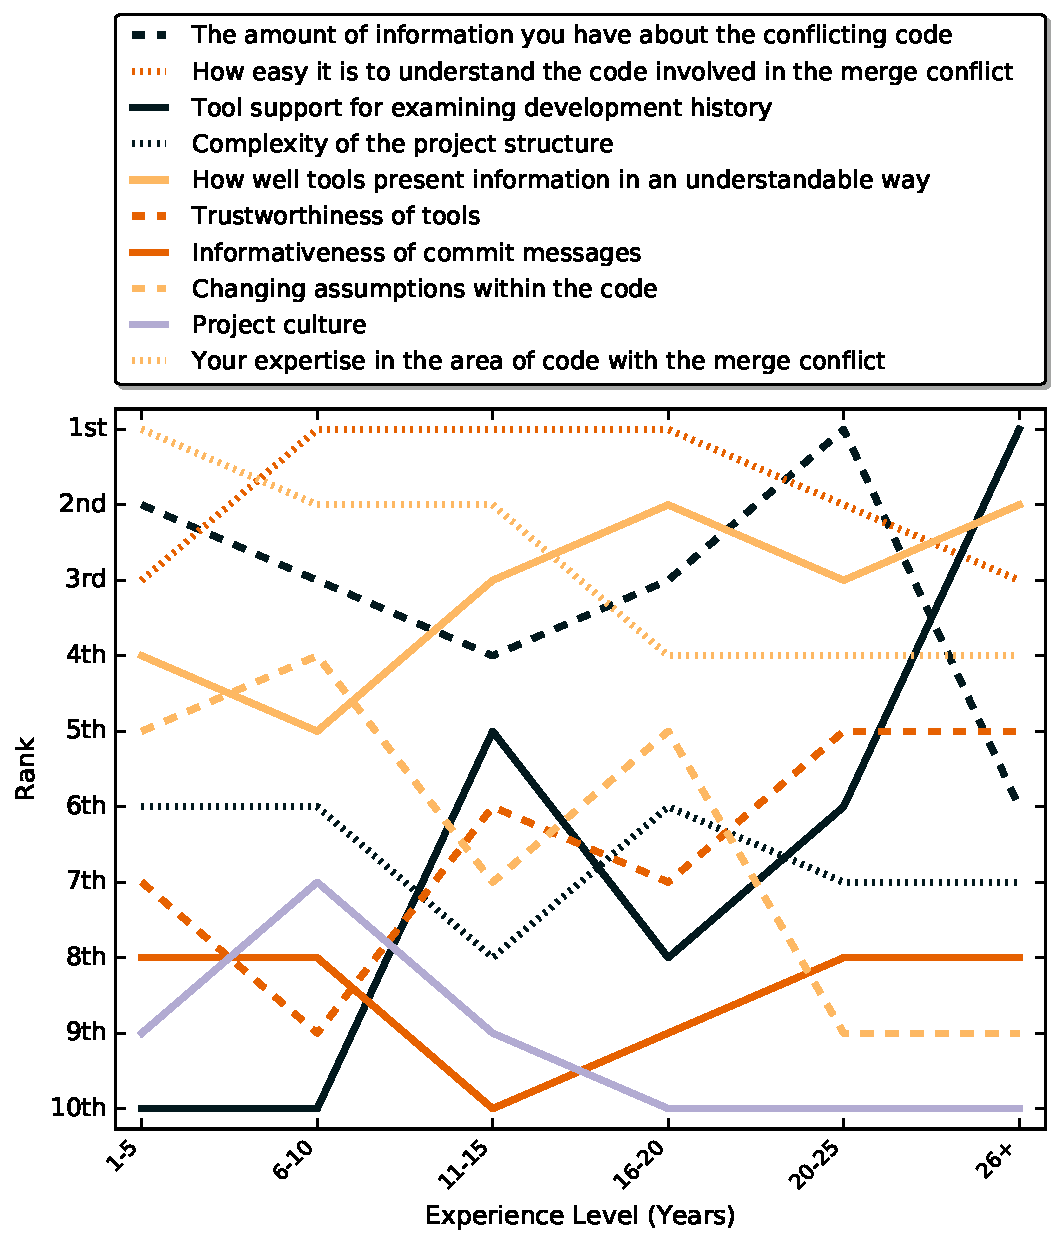
\includegraphics[width=2.5in]{ExpVsRankResDiff.pdf}
\caption{The rank of factors of difficulty during merge conflict resolutions by experience level}
\label{res_diff_rank}
\end{figure}

\subsubsection{Factors of difficulty in merge conflict resolution}

These individual factors emerged through the interview processing via the method of card sorting previously described. Of 141 responses, Figure \ref{res_diff_rank} shows the rank of each factor where the rank 1 factors into the difficulty of resolving a merge conflict the most, and the rank 10 affects the difficulty of merge conflict resolution the least.

Some key factors to consider in Figure \ref{res_diff_rank}:
\begin{itemize}
\item \textbf{Tool support for examining development history}\\
This factor starts out ranked as the factor that least affects the difficulty of a merge conflict resolution in the group of least experienced respondants.
\item \textbf{Another key point}\\
***Explanation*** 
\end{itemize}

\textbf{***Tool support for examining development history from 10th to 1st***}\\
\textbf{***Expertise in the area of code becomes less important (1-4) ***}\\
\textbf{***Project Culture generally not important, especially with more experience***}\\
\textbf{***commit message informativeness lower than expected***}\\

\begin{figure}[!t]
\centering
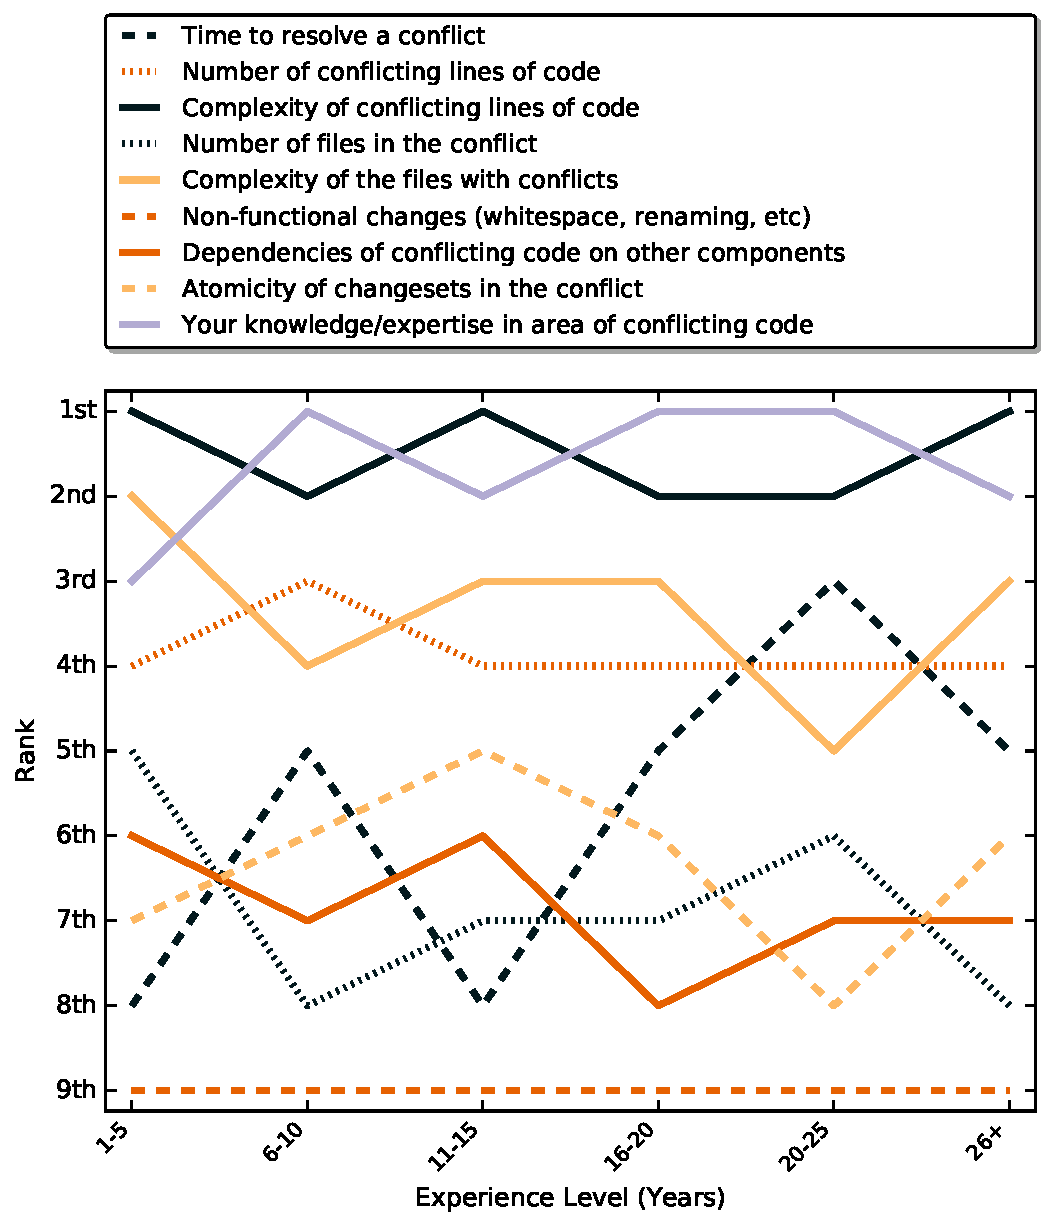
\includegraphics[width=2.5in]{ExpVsRankConDiff.pdf}
\caption{Rank of difficult factors in merge conflicts by experience level}
\label{con_diff_rank}
\end{figure}

\subsubsection{Factors of difficulty in merge conflicts}
Survey participants were asked...

\textbf{*** Complexity of conflicting lines of code is important***}

\textbf{***Knowledge or expertise in the area of conflicting code is important***}

\textbf{***Time to Resolve the conflict increased with Experience***}

\textbf{*** Non-functional changes don't matter to anybody ***}

\textbf{***How each demographic differs from the whole***}

\textbf{***Tool Trust. 42.1\% Trust their tools less than A Lot***}

When 121 participants of no particular role were asked how much they trust their merging, history exploration, and/or conflict resolution tools, 57.9\% of participants reported that they trusted these tools either A Lot or Completely. While this is a majority of developers, this still leaves a significant number of people (42.1\%) who trust their tools A Moderate Amount or A Little. While we found no previous work discussing the threshold for how much trust a user must have in a tool, it seems reasonable to postulate that users who cannot trust their tools A Lot or Completely will avoid relying on such tools or thoroughly check that the tools correctly performed their tasks. 

\begin{figure}[!t]
\centering
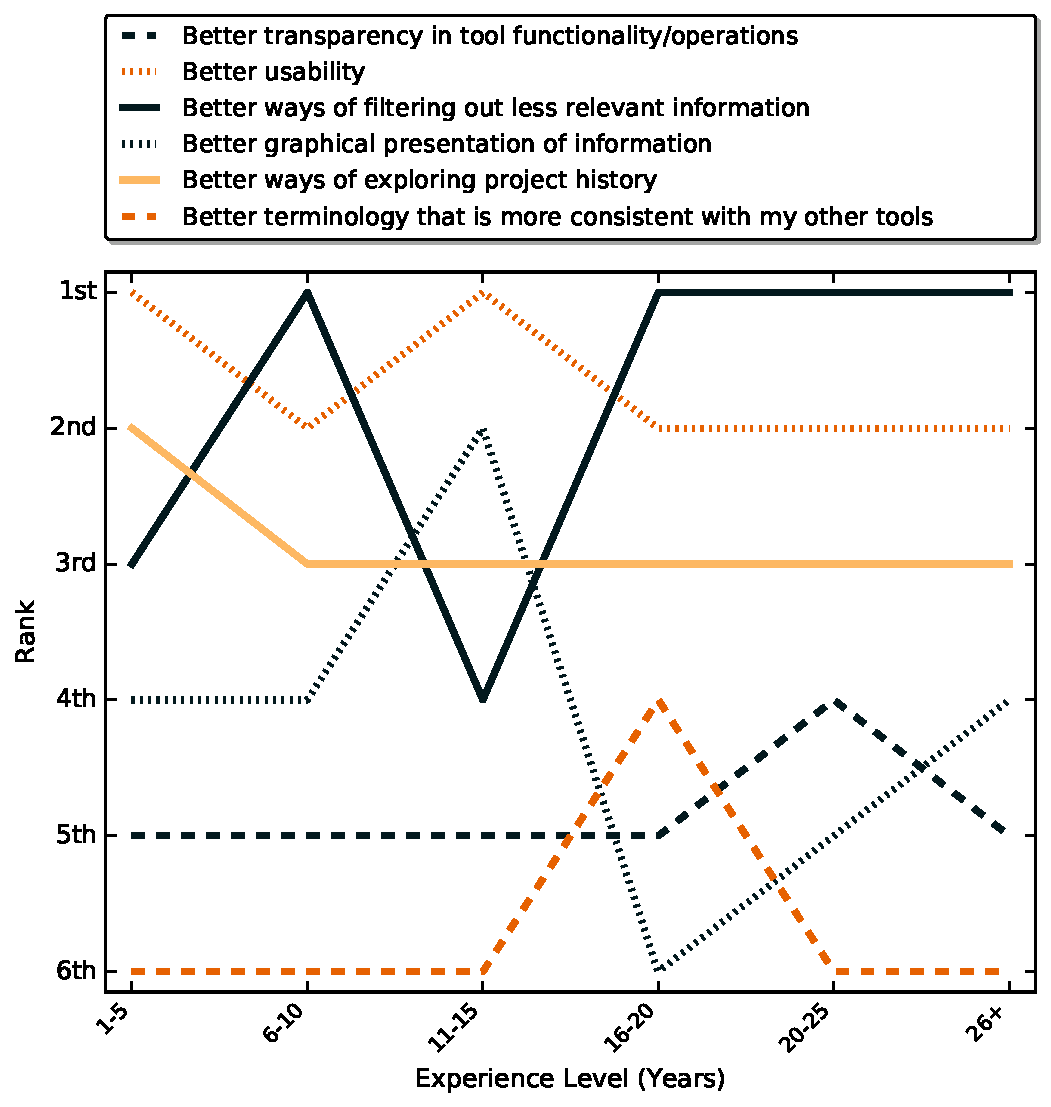
\includegraphics[width=2.5in]{ExpVsRankToolNeeds.pdf}
\caption{Rank of different tool needs by experience level}
\label{tool_needs_rank}
\end{figure}

\subsubsection{Tool Needs}
Survey participants were asked what kind of improvements they would like to see in their tools. Of the options extracted from interviews, Figure \ref{tool_needs_rank} shows the rankings of each factor based on its median value rated by developers at different experience levels.

\textbf{***Many of the results show a certain level of agreement across most experience levels. ***}

Though there is some variation, several of these factors are consistent across experience levels. For instance, every experience level considers "Better Usability" to be either 1st or 2nd priority, developers with more than 5 years of development experience rank "Better ways of exploring project history" as the 3rd priority, and 4 of 5 experience levels rank "Better transparency in tool functionality/operations" as 5th most important of 6 factors. 5 of 6 groups also showed little concern about improving terminology and its consistency across different tools.
Notably, more experienced developers agree that better ways of filtering out less relevant data is important

\textbf{***Usability is important***}

\textbf{***Most don't seem to care about terminology***}

\textbf{***Better graphical presentation  of information seems to mattter more for less experienced devs***}

\textbf{*** The most experienced groups want better wats to filter out less relevant information***}

\textbf{***People care less about the transparency in operations***}

\begin{table}[!t]
\renewcommand{\arraystretch}{1.3}
\caption{How much each factor affects the difficulty of a merge conflict resolution}
\label{percent_res_diff_table}
\centering
\begin{tabular}{c|c|c|c|c|c}
\hline
Factor & \multicolumn{5}{c}{ \% Respondents}\\
\hline
& A Great Deal & A Lot & A Moderate Amount & A Little & Not At All\\
\hline
How easy it is to understand the code involved in the merge conflict & 26.2 & 46.1 & 17.7 & 9.9 & 0\\
Your expertise in the area of code with the merge conflict & 25.5 & 34.8 & 27 & 12.1 & 0.7\\
How well tools present information in an understandable way & 24.1 & 22.7 & 33.3 & 17 & 2.8\\
The amount of information you have about the conflicting code & 22.7 & 34 & 27 & 14.9 & 1.4\\
Changing assumptions within the code & 17.7 & 25.5 & 31.9 & 19.1 & 5.7\\
Trustworthiness of tools & 17 & 22.7 & 27.7 & 20.6 & 12.1\\
Tool support for examining development history & 15.6 & 22.7 & 22 & 28.4 & 11.3\\
Project culture & 14.9 & 19.1 & 30.5 & 26.2 & 9.2\\
Complexity of the project structure & 12.1 & 29.1 & 27.7 & 27 & 4.3\\
Informativeness of commit messages & 12.1 & 31.2 & 21.3 & 22.7 & 12.8\\
\hline
\end{tabular}
\end{table}

\section{Discussion}
\subsection{Implications}
\subsubsection{For Researchers}
\subsubsection{For Tool Builders}
\subsubsection{For Developers}


\section{Conclusion}
The conclusion goes here.

\section*{Acknowledgment}

The authors would like to thank Alex Hoffer, Iftekhar Ahmed, Michael Hilton, Sruti Ragavan, and all of our interview and survey participants, especially those who helped distribute interview requests and survey links.

\begin{thebibliography}{1}

\bibitem{IEEEhowto:kopka}
H.~Kopka and P.~W. Daly, \emph{A Guide to \LaTeX}, 3rd~ed.\hskip 1em plus
  0.5em minus 0.4em\relax Harlow, England: Addison-Wesley, 1999.

\end{thebibliography}




% that's all folks
\end{document}


